% !TEX root = paper.tex 
\section{Motivation and Relevance}

Digital wireless communication has become irreplaceable in our modern information technology and society. Communication is done primarily “on the go” using smartphones instead of cable bound landlines. The trusty Ethernet-port is disappearing in modern ultra-slim notebook computers, instead networks are accessed solely via Wi-Fi (IEEE 802.11). Even some household devices such as fridges or even dishwashers can be connected to the internet via Wi-Fi.

Developments like these do no only lead to a world full of exciting new possibilities, but also to a tremendous amount of new potential security risks. Hackers can and do use the ever-growing amount of unsecure or badly secured wireless networks for their own illicit purposes, such as ordering illegal goods or obscuring their access point, or just surfing the internet for free without paying a service provider to access to their infrastructure.  

The reasons to break into a secured wireless network however do not necessarily have to be illegitimate. In fact, the best way to verify a security concept and implementation is to attack it in a controlled and documented manner --- the art of \emph{Penetration testing}.

\section{Testing setup}

To avoid legal issues, a controlled testing setup was constructed for the purpose of this research:

\begin{itemize}

\item{Lenovo Y50-70 \textbf{Laptop} running Kali Linux~\cite{OffSec17} inside a virtual machine}

\item{TP-LINK TL-WN722N \textbf{USB-WiFi antenna}}

\item{TP-LINK TL-WR542G \textbf{wireless router}}

\item{Samsung ATIV-S \textbf{Smartphone} running WP 8.1}

\end{itemize}

A USB antenna was chosen for its extended range and higher transmitting power, compared to the laptops' integrated Wi-Fi antenna. This is especially important when performing attacks where overshadowing another network is the key to successful attack, as shown in Section~\ref{sec:attackuser}.

The operation system \emph{Kali Linux} by \emph{Offensive Security} is a Linux Debian-based system that was initially released in March 2013 as a successor to BackTrack Linux~\cite{OffSecDoc17}. Kali Linux was chosen for its flexibility and vast collection of pre-installed penetration testing software.

Any other devices were already owned and thus chosen because of their availability.

\subsection{Used software}

Kali Linux provides a massive collection of software, engineered for all kinds of use cases. A few specialized programs were used for the purpose of this research:

\begin{itemize}

\item{\textbf{Aircrack-ng suite}~\cite{AirNg17}, capable of using network cards in monitoring mode, capturing packets, decrypting captured traffic and even running active attacks such as deauthentication or packet injection}

\item{\textbf{John the ripper}~\cite{Openwall17}, an advanced password-cracking and hash-breaking tool to use with aircrack-ng}

\item{\textbf{Fluxion}~\cite{Fluxion17}, a WPA phishing framework which provides a user-friendly interface and is capable of launching Man-in-the-Middle attacks}

\item{\textbf{Reaver}~\cite{Reaver17}, a brute-force WPS PIN cracker}

\end{itemize}

\subsection{Wireless adapter configuration}\label{sec:wificonf}

A Wi-Fi adapter generally can be operated in a multiple distinct modes, \emph{monitor} and \emph{managed} modes. Most household and end-user devices operate in a managed mode, where the networking card acts as a client or access point. In managed mode, the hardware filters the incoming packets before they are forwarded to the operation system. 

Configuring the network card to operate in monitor mode lets the received packets bypass the internal processing unit of the network card and allows the CPU to process the raw packets instead. Also, in monitor mode the network card does not have to be associated to an existing wireless network, making it possible to capture foreign and broken packets or even inject new packets into the network.

Using the above-mentioned aircrack-ng suite, setting the wireless card to monitoring mode can be done by the systems' super user by running

\begin{lstlisting}[basicstyle=\ttfamily]
airmon start wlan0
\end{lstlisting}

With \lstinline[basicstyle=\ttfamily]{wlan0} being the desired networking interface. This command will then create an new network interface, \lstinline[basicstyle=\ttfamily]{wlan0mon}, which exposes the monitoring capability. This can be verified by checking the output of the command \lstinline[basicstyle=\ttfamily]{iwconfig}.

Not all wireless adapters, drivers and operating systems support using the adapter in monitoring mode. The above configuration has been shown to fulfill all expectations.

\section{WPS-secured networks}

Wi-Fi Protected Setup, or \emph{WPS} for short, is a protocol which aims to simplify the process of adding new devices (hereinafter called \emph{Enrollee}) to a wireless network provided by a wireless router (hereinafter called \emph{Registrar}). 

Usually, when using a traditional protocols such as WEP or WPA, the user must enter a password in order to authorize a device. WPS on the other hand allows several quick methods to authorize a device~\cite{WiFi11}, all being based on physical access to the router:

\begin{itemize}

\item{Entering a pre-determined eight digit long \textbf{Personal Indentification Number} (PIN) into the new device. This PIN is often printed on the router itself and is comparable to a regular password. 

However, some models possess a vulnerability where the PIN is derived from the routers' MAC address~\cite{Craig14}, which can be sniffed.}

\item{Via the \textbf{Push Button Configuration} (PBC), where pressing a dedicated hardware button on the router allows new connections for two minutes (See Figure~\ref{fig:wpsbutton}). }

\item{Transferring configuration data using a \textbf{USB Flash Drive} (UFD) from the router to the new device.}

\item{Via \textbf{Near Field Communication} (NFC) where data exchange is achieved by close-range electromagnetic induction.}

\end{itemize}

\begin{figure} %[H]
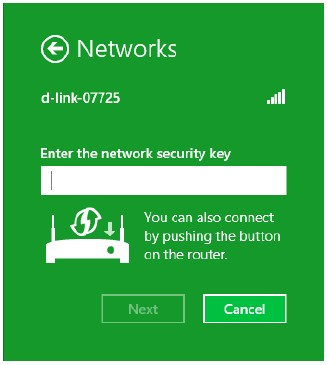
\includegraphics[width=0.3\textwidth]{src/img/DIR-890L-WPS-Button-windows-8c.jpg}
\caption{Connecting to a WPS network in Microsoft Windows 8. From D-Link~\cite{DLink14}}\label{fig:wpsbutton}
\end{figure}

\subsection{Reduced PIN compexity}\label{sec:wpsredpin}

While an eight-digit PIN in itself is already possible to be brute-forced, several flaws in WPS reduce the amount of guesses needed further down~\cite{Ducklin15}. 

Firstly, the last digit of the PIN is a check digit, which can be computed from the other seven. Furthermore, authorization of the enrollee is done in multiple steps~\cite{WiFi06}, in which the enrollee proves possession of the PIN in two stages, one for each half of the PIN (see Table~\ref{tbl:wpskey}).

Because authorization prematurely fails after an invalid first half of the PIN, an attacker only has to guess $10^4 + 10^3$ times assuming the worst case --- as opposed to the original $10^8$ times.

\begin{table}[]
\centering
\caption{Composition of a WPS Key}\label{tbl:wpskey}
\begin{tabular}{l|c|c|c|c|c|c|c|l|}
\cline{2-9}
 & \multicolumn{8}{c|}{PIN} \\ \cline{2-9} 
Digit & 1 & 2 & 3 & 4 & 5 & 6 & 7 & \multicolumn{1}{c|}{8} \\ \cline{2-9} 
 & \multicolumn{4}{c|}{First half} & \multicolumn{3}{c|}{Second half} & C \\ \cline{2-9} 
\end{tabular}
\end{table}

\subsection{Flawed random number generator}

Some routers implemented a weak random number generator, which enabled hackers to launch an effective \emph{offline} brute-force attack against captured data from the (failed) WPS PIN handshake~\cite{Bongard14}, called the \emph{Pixiedust} vulnerability.

However, the test device and nearly all devices released within the last few years did not possess this characteristic, so further evaluation was discontinued for the purpose of this research.

\subsection{Attacking with Reaver}

The \emph{Reaver} password cracker can be used to perform the attack described in Section~\ref{sec:wpsredpin}, after the wireless network adapter has been properly initialized as described in Section~\ref{sec:wificonf}:

\begin{lstlisting}[basicstyle=\ttfamily]
reaver -i wlan0mon -c 6 -b 00:19:E0:6E:C4:DE -vv
\end{lstlisting}

With \lstinline[basicstyle=\ttfamily]{6} being the wireless channel in with the router operates, and \lstinline[basicstyle=\ttfamily]{00:19:E0:6E:C4:DE} the routers' MAC address. 

This information can be found by scanning the network for wireless access points, for example using \lstinline[basicstyle=\ttfamily]{wash -i wlan0mon} or \lstinline[basicstyle=\ttfamily]{airodump-ng wlan0mon}. Reaver will then brute-force the WPS PIN, and display it when successful. 

Without special mitigation tactics this process can take up to a few hours, or just a few minutes when a \emph{Pixiedust} vulnerability is detected.

\section{WEP-secured networks}

Wired Equivalent Privacy, or \emph{WEP} for short, is a deprecated jet still used Wi-Fi authorization and encryption protocol.

Data is encrypted by XOR-ing it with a pseudorandom stream of data (see Figure~\ref{fig:wepmech}), which is generated using the RC4-Algorithm~\cite{WiFi16}.

The RC4 random number generator is initialized with the concatenation of an 24-bit \emph{Initialization Vector} (IV) and the actual hexadecimal password. The width of the seed can range from 64 to 256 bits in some implementations.

\begin{figure}
\includesvg{src/img/Wep-crypt-alt.svg}
\caption{Basic WEP encryption mechanism. From Wikipedia, the free encyclopedia~\cite{BHL07}}\label{fig:wepmech}
\end{figure}

\subsection{Related-Key vulnerability}

The RC4 random number generator is vulnerable to the \emph{Fluhrer, Mantin and Shamir attack}~\cite{FMS01}.

Using certain generated IVs, an attacker can --- knowing the first byte of the key stream and the first n bytes of a key --- derive the next byte of this key.

To receive enough (a few thousand) IVs, an attacker has to choose a rather busy network and/or collect packets for a long period of time.

This information can then be used to deduce the original key und consequently the password.

\subsection{Increasing the amount of IVs}

% when are iv generated
% arp
% arp fuckery

\subsection{Attacking with Aircrack}

\section{WPA2-secured networks}

Theory

Attack

Practice

\section{Social engineering}\label{sec:attackuser}

Humans are, compared to computer-based authorization algorithms, rather gullible. 

Phishing

Social Engineering

\section{Conclusion}

Wrapping up, there really is no way to provide 100\% unbreakable wireless network security. However, it is possible to make it extraordinarily hard for an attacker to breach a network. 

This can be done on the technical side by:

\begin{itemize}

\item{Disabeling deprecated protocols like WEP and WPS and upgrading to WPA2}

\item{Picking long and complex pre-shared-keys and passwords}

\item{Keeping the wireless routers' firmware up-to-date}

\item{Restricting physical access to the wireless router}

\end{itemize}

And on the social side by:

\begin{itemize}

\item{Educating users about phishing and social engineering attacks}

\item{Demonstrating attacks to sensitize users to tell-tale signs of such attacks}

\item{Implementing strict password policies}

\item{Using a per-user authentification system}

\end{itemize}